\documentclass[11pt,a4paper,finnish,oneside]{article}
\usepackage[utf8]{inputenc}     % Linux
%\usepackage[ansinew]{inputenc} % Windows 
\usepackage[T1]{fontenc}
\usepackage[finnish]{babel}
\usepackage[left=4cm,right=4cm,top=3cm,bottom=3cm]{geometry}
\usepackage{graphicx}
\usepackage{color}
\usepackage{epstopdf}


\usepackage{subfig}



\sloppy
\definecolor{lightgray}{gray}{0.5}
\setlength{\parindent}{0pt}

\begin{document}
\begin{titlepage}  
\title{Graduaiheiden hallintajärjestelmä}
\author{(tsoha)}
\date{\today}
\maketitle    
\tableofcontents
\end{titlepage}    


\section{Johdanto}

\begin{par}
Graduaiheiden hallintajärjestelmä on tarkoitettu helpottamaan sitä monen toimijan keskinäistä koordinaatiota, jota hyvän graduaiheen löytäminen edellyttää. Se mahdollistaa niin opiskelijoiden kuin opettajienkin selvittää, millaisia graduja on tehty, tai työn alla, ja kenen ohjauksessa. Nämä tiedot taas auttavat sopivien aiheiden ja ohjaajien etsinnässä, ja mm. päällekkäisyyksien välttämisessä.
\end{par}\vspace{1em}

\begin{par}
Järjestelmällä on erilaisia käyttäjiä. Opiskelijat ja ohjaajat voivat etsiä millaisia aiheita on työn alla, kenen ohjauksessa, ja millaisia graduja on jo tehty. Ohjaajat voivat opiskelijan kanssa gradunteon aloittamisesta sovittuaan lisätä sovitun aiheen järjestelmään, ja sen jälkeen muokata sitä halunsa mukaan. Ohjaajan vastuuseen kuuluu myös luokitella aihe johonkin/joihinkin yleistasoiseen luokkaan, ja ohjaaja voi liittää aiheeseen tietoja sen edistymisestä. Kaikki edistymistiedot eivät näy opiskelijoille.
\end{par}\vspace{1em}

\begin{par}
Järjestelmä toteutetaan tietojenkäsittelytieteen laitoksen users-palvelimella Tomcat- tai Apache-palvelimen alla. Alustajärjestelmän on tuettava PHP -ohjelmointikieltä ja järjestelmän käyttäjän selaimen javascriptiä. Käytettävän tietokannan on oltava PostgreSQL olio-relaatiotietokannan.
\end{par}

\section{Käyttötapaukset}
\subsection*{Käyttötapauskaavio}


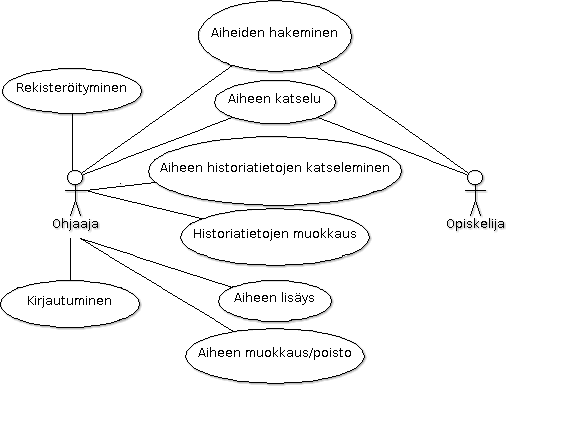
\includegraphics [width=6in]{useCase1.png}
\vspace{2em}

\subsection*{Käyttäjäryhmät}
\begin{par}
\begin{description}
\item[Opiskelijalla]tarkoitetaan käytännössä ketä tahansa henkilöä, jota kiinnostaa tietää, millaisia graduja on tehty ja/tai tekeillä. Nämä henkilöt ovat potentiaalisia tai aktuaalisia opiskelijoita.
\item[Ohjaaja] on laitoksen graduohjaaksi hyväksymä henkilö, jolla on ollut/ on tällä hetkellä graduja ohjattavanaan, ja jonka ohjaajan ominaisuudessaan tarvitsee merkitä järjestelmään graduaiheita sekä päivittää niitten tietoja.
\end{description}
\end{par}
\subsection*{Käyttötapauskuvaukset}
\begin{par}
\subsubsection*{Opiskelijan käyttötapaukset}
Aiheiden hakeminen:
\begin{itemize}
  \item[]Opiskelija hakee graduaiheita aiheluokan tai ohjaajan perusteella. Hakutuloksena otsikoita sekä vuosilukuja.
\end{itemize}
Aiheen katselu:
\begin{itemize}
  \item[]Opiskelija katsoo graduaiheeseen liittyvät tiedot, jotka hänen on mahdollista nähdä. Valmiista graduista tekijän nimi, keskeneräisistä ainoastaan ohjaajan.
\end{itemize}

\subsubsection*{Ohjaajan käyttötapaukset}
Aiheen lisäys:
\begin{itemize}
  \item[]Ohjaaja lisää (yhteistyössä opiskelijan kanssa) graduaiheen, jonka on ottanut ohjattavakseen, liittäen siihen tiedon sen tekijästä sekä luokitellen sen johonkin yleistasoiseen luokkaan. Otsikko ja suunniteltua sisältöä valaiseva kuvaus.
\end{itemize}
Aiheen muokkaus/poisto:
\begin{itemize}
  \item[]Ohjaaja muokkaa aiheen otsikkoa, kuvausta tai sen historiatietoja. Ohjaaja voi myös poistaa aiheen.
\end{itemize}
Aiheen historiatietojen katseleminen
\begin{itemize}
  \item[]Ohjaaja katsoo aiheeseen liittyviä historiatietoja, kuten tekijää koskevia tietoja, ja gradun edistymistä koskevia tietoja. Ajankohtia kuten graduseminaarin suorittamisaika, tarkastukseenjättämisaika jne. 
\end{itemize}
Muita tapauksia: Kirjautuminen, aiheiden haku, aiheen katselu.

\end{par}\vspace{1em}


\end{document}
    
